\section{Measured one-run reliability}
\label{sec:results}

\paragraph{Completed coverage and reference checks.}
All nine fitted dataset/model cells completed the frozen panel: 540 exact empirical-game references and 97,200 stochastic calls, with 60 inputs and 30 independent seeds per estimator/budget condition. The saved-vector audit verified the full grid, unique seeds, frozen source identity and recorded primary metrics. No failed attempts, warnings, rank-deficient Kernel designs or exhaustive primary calls were recorded. Maximum reference and stochastic efficiency residuals were $6.66\times10^{-16}$ and $8.88\times10^{-16}$ probability units. These residuals supplement the independent implementation checks in Appendix~\ref{app:implementation-checks}; they are not standalone coordinate-accuracy proofs. Held-out ROC AUC ranges from $.823$ to $.852$ on German Credit, $.885$ to $.896$ on ACSIncome and $.879$ to $.894$ on Diabetes. These diagnostics describe the fitted predictors, not the correctness of their rationales.

Figure~\ref{fig:one-run-budget} shows adequacy against actual prediction work; Figure~\ref{fig:criterion-instance-contrast} contrasts stricter recovery and input-level failures. The matched-scale reference-error/run-disagreement display (Figure~\ref{fig:error-repeatability}), CPU curves and complete condition/component/instance displays and tables are in Appendix~\ref{app:numerical}.

\begin{figure}[tb]
\centering
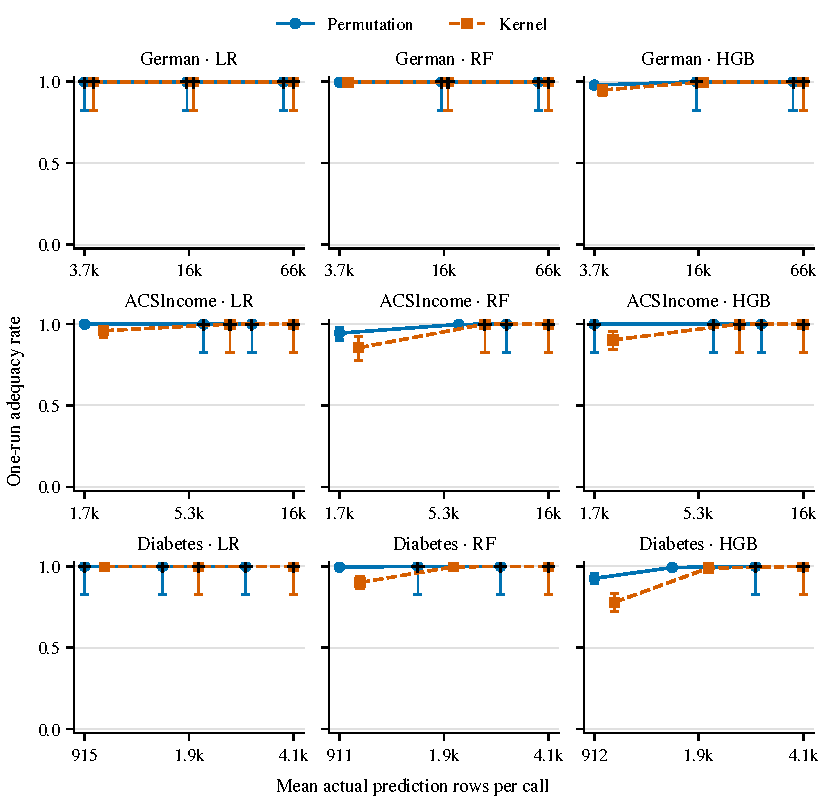
\includegraphics[width=\linewidth]{figures/one_run_budget.pdf}
\caption[One-run adequacy versus actual prediction work.]{One-run adequacy: normalized L1 error $\leq$0.20 and signed top-3 overlap $\geq$2/3 against the exact finite-game reference. L1 normalization is max(reference L1,0.01 probability units). For each fixed fitted model, 60 held-out inputs and 30 independent runs per input, estimator and requested budget; background B=32. The target is positive-class probability for the fixed empirical interventional game over grouped raw features. Estimates average equally over inputs and runs. Bars are analysis-supplied pointwise 95\% instance-cluster percentile intervals, conditional on the fitted model, split and background. Black plus markers identify observed all-zero/all-one panels whose displayed bars instead use the supplied two-sided 95\% bounded-instance Hoeffding interval. These are observed rates and descriptive intervals, not population 95\% adequacy certification. Horizontal positions are mean measured prediction rows; nominal budget equality does not imply equal actual work.
}
\label{fig:one-run-budget}
\end{figure}

\paragraph{Finite-budget failures and improvements.}
For the declared event, lowest-budget Kernel success varies from $.7794$ to $1$ across the nine fitted cells; permutation success varies from $.9261$ to $1$. Diabetes histogram boosting with Kernel at budget 32 is the lowest observed condition: $.7794$ with pointwise 95\% interval $[.7217,.8345]$. ACS forest with Kernel at budget 64 achieves $.8544$ $[.7767,.9233]$, and German histogram boosting at budget 128 achieves $.9494$ $[.9133,.9800]$. The differences across these fixed predictors show why a single pooled success rate would conceal useful conditions. Logistic probability explanations also remain stochastic: for example, ACS logistic Kernel at budget 64 achieves $.9589$ $[.9200,.9883]$.

Increasing work improves the difficult low-budget conditions. For Diabetes histogram boosting with Kernel, budget 32 minus budget 128 has paired-input adequacy difference $-.2206$, interval $[-.2783,-.1655]$. All eighteen highest-budget estimator/model conditions have observed primary success $1$: each has 1,800 calls on 60 input clusters, rather than 1,800 independent inputs. Their displayed boundary-adjusted intervals are $[.8247,1]$. This wider boundary interval reflects the predeclared conservative treatment, not a decline in the observed success or an estimate of zero sampling uncertainty. None clears the separate population-success guard at $.95$.

\paragraph{The numerical reading changes the answer.}
The primary criterion permits one of the three signed salient features to differ. Requiring all three, at the same $.20$ magnitude tolerance, reduces highest-budget observed success to between $.9289$ and $1$. The lowest such strict result is Diabetes histogram boosting with permutation, $.9289$ $[.8967,.9589]$. Thus high-budget success for the two-of-three reading does not mean exact feature-list recovery. Component, error-cutoff, strict-selection and tie-aware outputs accompany the main event; magnitude-only adequacy must not be described as joint adequacy.

Panel success also conceals individual difficulty. ACS forest Kernel at budget 64 has one held-out input (panel index 30, with its original source row retained in the results) with 0/30 adequate runs. Its per-input Wilson interval is $[0,.1135]$, despite the panel estimate $.8544$. This case was found retrospectively; it is evidence for displaying input-level variation, not a prospectively validated rule for identifying unreliable inputs. Conversely, thirty successful seeds on another input would not establish absence of rare failures.

\paragraph{Repeatability is a separate measured property.}
Pairwise disagreement and reference error use the same reference-norm floor, with all run pairs reduced to one input summary. Their agreement events still ask different questions. ACS forest Kernel at budget 64 has one-run reference adequacy $.8544$, whereas pairwise joint agreement is $.7207$ $[.6239,.8085]$. This example does not show that reassuring repeatability concealed error; here pairwise agreement is lower. It shows that the two probabilities are not interchangeable. Full vector and signed-selection summaries preserve both assessments, without treating shared run pairs as independent observations. Averaging thirty runs is separately available with its thirty-run cost; its accuracy cannot be credited to one run.

\begin{figure}[tb]
\centering
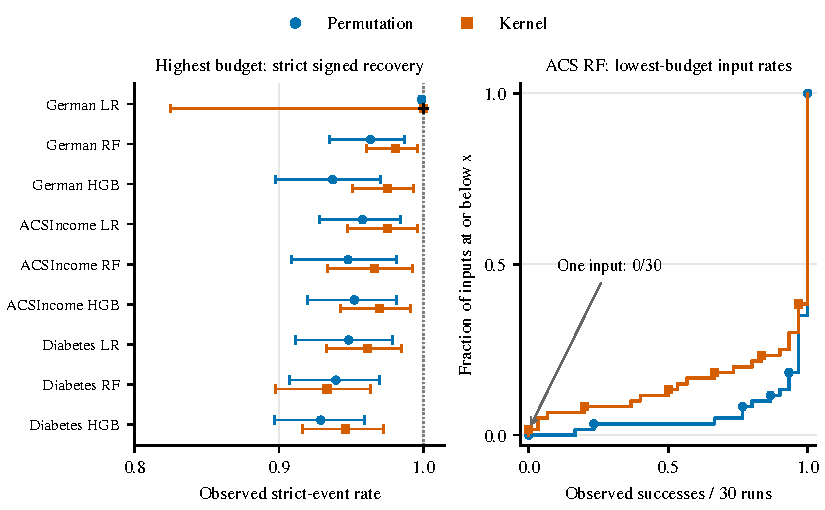
\includegraphics[width=\linewidth]{figures/criterion_instance_contrast.pdf}
\caption[Criterion and input dependence of observed adequacy.]{Criterion and input dependence. Left: the strict event at the highest requested budgets (German 2048, ACS 512, Diabetes 128) requires normalized L1 <=0.20 and all three signed top-3 features matching the exact reference. Broad two-of-three primary-event rates are observed 1 for all these conditions, with supplied boundary interval [0.824670,1]; they do not imply exact feature recovery or population >=0.95 certification. Strict-event bars are supplied pointwise 95\% instance-cluster percentile intervals; black plus marks denote the supplied two-sided Hoeffding replacement at an observed all-success boundary. Each condition has 60 inputs and 30 independent runs/input. Right: ECDF of observed primary-event input success fractions for ACS RF at requested budget 64; means can hide poor individual observations. Kernel input 30 (original source row 296124) has 0/30 successes, with supplied Wilson interval [0.000,0.114]. The ECDF has no confidence band and is not the distribution of known latent input probabilities. All panels condition on fixed fitted models, split and B32 empirical interventional probability game over raw-feature groups, with L1 normalization max(exact-reference L1,0.01). No individual certificate or equal-cost superiority follows.
}
\label{fig:criterion-instance-contrast}
\end{figure}

\paragraph{Which failure conditions were observed?}
Budget, fitted predictor and the requested numerical reading distinguish observed success from failure in this panel. The prespecified near-top-one-gap stratum contains only 2--21 inputs per fitted cell. For example, lowest-budget ACS forest Kernel success within its four near-gap inputs is $.6500$ $[.4417,.8917]$; other cells do not show a uniform gap effect. These descriptive strata neither establish a mechanism nor validate a general risk classifier. No reference-defined low-signal input, numerical top-one/top-three boundary tie or selected near-zero sign was observed. The minimum reference L1 norm is $.07588$, above all tested floors $.001/.01/.05$; those floor choices therefore give identical results. Low-signal behavior remains untested, rather than demonstrated harmless. Stable index ordering defines exact point scores, and the reported ambiguity counters disclose where numerical tolerance could have affected their interpretation.

\paragraph{Changing the background changes the target.}
A separate arm retains twelve main inputs per fitted ACS/Diabetes model and compares B8/B128 training-row backgrounds at the middle budget, with twenty seeds per estimator and exact changed targets (Appendix~\ref{app:background}). For ACS logistic B8, the mean exact-target shift from B32 is $.4977$ normalized L1, interval $[.4335,.5641]$, although both estimators have observed success $1$ against that new exact target. This is conditional target sensitivity: B32 is not population truth, and one draw per size confounds size with row resampling. Its 144 references and 5,760 calls remain outside the primary repetition estimand.

\paragraph{Actual computation and interrupted elapsed clocks.}
Main jobs used 7.493 CPU hours: 5.659 for exact references, 1.779 for stochastic calls and $.0556$ for the remaining process overhead. The pre-run main projection was 7.405 CPU hours; pilots, statistical postprocessing and the separate background arm are outside this measured main total. Peak main process RSS was 831,824 KiB. Across named conditions, mean one-run CPU costs range from $.000638$ to $.339$ seconds and mean prediction work from about 911 to 65,569 model-input rows. These are condition means, not service-latency limits or individual maxima. Exact references dominate study cost and are not needed for every production explanation once an assessment has been performed.

Across the disjoint recorded main, preliminary, development and background intervals, the measured subtotal is 7.835 CPU hours. Several setup, failed-control, validation and postprocessing intervals lack CPU timers; their unknown costs are not zero, and this subtotal is not an exact whole-study total (Appendix~\ref{app:reproduction}).

Equal nominal budgets do not execute equal work: paired integer paths, within-run caching and endpoint/background expansion change prediction rows and CPU costs. The supplied paired nominal-budget contrasts therefore cannot establish equal-cost superiority. Recorded wall times are preserved, including severe interruptions: two German reference calls each exceed 162,000 elapsed seconds while using under 180 CPU seconds. Process CPU and actual rows are the primary efficiency currencies; these interrupted wall clocks describe this execution and cannot serve as a clean deployment-latency benchmark. Overlapping cell elapsed times are not added into a study duration.
